\documentclass[10pt,a4paper]{article}
\usepackage[utf8]{inputenc}
\usepackage{amsmath}
\usepackage{amsfonts}
\usepackage{amssymb}
\usepackage{natbib}
\usepackage{graphicx}
\usepackage[left=2cm,right=2cm,top=2cm,bottom=2cm]{geometry}
\usepackage{arydshln}
\begin{document}

\section{Introduction}\label{sec:Introduction}

Crustal strain rates are fundementally important quantities for assessing seismic hazard. This is because the locations where strain is rapidly accumulating are the locations where we can expect strain energy to be released seismically.  It is then important to develop and improve upon methods for mapping strain in tectonically active regions because such maps could concievably feed into seismic hazard models such as UCERF3 \citep{Field2014}. 

Maps of strain rate can be derived from geodetic measurements of ground displacements, and there are numerous methods for doing so.  The classic and simplest way is to assume that the strain rate is constant in time and spatially uniform within subnetworks of the geodetic data.  Linear least squares is then used to find the components of the strain rate tensor for each subnetwork \citep[e.g][]{Frank1966,Prescott1976,Savage1986,Feigl1993,Murray2000}. Several algorithms have been developed to improve upon this procedure for calculating strain. \citet{Shen1996} and \citet{Shen2015} discuss an algorithm where, instead of using the immediately adjacent stations to calculate strain at a position, the strain is computed with a weighted average over the entire network where the weighting is smaller for more distant stations.  Another strategy is to fit a set of interpolating basis functions to the velocity field and then compute the strain from the analytical derivative of the interpolant \citep[e.g.][]{Beavan2001,Tape2009}.  The aforementioned studies have all been concerned with estimating long term strain rates.  Time dependent strain would be useful for studying geophysical processes which occur over timescales of days to years such as slow slip events, postseismic relaxation, or volcanic deformation.  \citet{Ohtani2010} describes a Kalman filter based method for computing time dependent strain by fitting a set of basis functions to a time dependent displacement field and enforcing temporal smoothness in the basis function coefficients.   

In essence, estimating strain rates is a matter of numerically calculating the spatial derivative of a geodetically observed velocity field.  Any method proposed for calculating strain rates must be able to handle two complications; 1) geodetic velocity estimates are noisy and differentiation will only amplify the noise and 2) velocities are not observed on a regular grid, which prevents the use of standard finite difference methods for computing derivatives.  In this paper we demonstrate that both of these complications can be elegantly handled with the recently popularized Radial Basis Function-Finite Difference (RBF-FD) method \citep{Wright2006}.  

The RBF-FD method was introduced as an computationally efficient way to solve large scale partial differential equations over irregular, multi-dimensional domains.  The RBF-FD method can be thought of as a generalization of the traditional finite difference method, where the node layout is no longer restricted to regular grids. Indeed, the RBF-FD method can be used to estimate derivates of discrete data located at arbitrary scattered positions in multi-dimensional space.  The RBF-FD method is particularly appealing because it is algorithmically simple, regardless of the domain shape or node layout, and also because the method has performed well in numerous benchmark tests \citep[and references therein]{Fornberg2015}.

In this paper, we do not use the RBF-FD method to solve a partial differential equation, but rather we use it to spatially smooth and differentiate GPS derived velocity data.  Our smoothing strategy can be viewed  as a low-pass filter for scattered data where the degree of smoothness is controlled by a user specifies cutoff frequency.  This can be contrasted with interpolation based smoothing strategies \citep[e.g.][]{Howell2016} where the resulting interpolant can be largely and unpredictably controlled by the choice of basis function.  After spatially smoothing the velocity field we differentiate it with the RBF-FD method to get a strain rate map.  We also demonstrate that this procedure can be used to estimate time dependent strain rates.  In that case, we first temporally smooth and differentiate GPS displacement time series to get time dependent velocities.  We then spatially smooth and differentiate the resulting velocities for each time epoch.  

The method proposed in this paper has numerous advantages which set it apart from other methods for computing strain rates. The method is computationally efficient and stable (there is no inversion of an ill-conditioned matrix).  There are no hyper parameters or penalty parameters that need to be tuned for each application.  As opposed to interpolation strategies such as \citet{Beavan2001}, \citet{Tape2009}, or \citet{Ohtani2010}, our method assumes that velocities are locally rather than globally continuous, which allows us to easily handle discontinuities resulting from, for example, a creeping fault. 

We begin this paper by summarizing the RBF-FD method and explaining how we construct differentiation matrices for scattered data. We then introduce the smoothing strategy, which is applied to the observed geodetic data prior to differentiation.  We then provide two real world demonstraitions of our method for calculating strain rates.  First we calculate the long term strain rates in Southern California from the CMM3 velocity data set \citep{Shen2011}, and we verify that our results are consistent with other studies. We then calculate time dependent strain rates in Cascadia from the GPS data provided by UNAVCO.  In Cascadia, we analyze strain resulting from slow slip events and compare it to the long term tectonic strain accumulation. Slow slip events are found to produce compression in the Olympic Peninsula, which is in addition to the compression resulting from tectonic loading.  Further south in Oregon, the slow slip events tend to release the compressional strain that is accumulated tectonically.  While similar conclusions have been drawn from fault slip inversions for slow slip events, it is important to recognize that slip inversion are the product of inverting an ill-conditioned matrix making it difficult to determine whether slip inferences are real or just an artifact of the inversion.  The strain rates presented in this paper are more direct observations and can be interpretted with a higher degree of confidence. 

\section{Method}\label{sec:Method}
\subsection{Differentiating Scattered Data}\label{sec:Differentiating}

In this section we briefly summarizing the RBF-FD method and we refer the reader to \citet{Wright2006} or \citet{Fornberg2015} for additional details. Consider a set of nodes $\mathbf{x} = \{x_1, ..., x_N\}$ in $\mathbb{R}^d$ and a corresponding vector $\mathbf{u} = [u(x_1), ..., u(x_N)]^T$.  We want to find a differentiation matrix $\mathbf{L}$, such that $\mathbf{Lu}$ approximates the linear differential operator $\mathcal{L}$ acting on $u$ at $\mathbf{x}$.  For each node $x_i$ we approximate $\mathcal{L}[u(x)]\big|_{x=x_i}$ as a weighted sum of $\{u(x_j): j \in \mathcal{S}_i\}$ where $\mathcal{S}_i$ consist of $i$ and the indices for the $n-1$ nearest neighboring nodes to $x_i$.  The approximation can be written as

\begin{equation}\label{eq:RBFFDApprox}
\mathcal{L}[u(x)]\big|_{x=x_i} \approx \sum_{j \in \mathcal{S}_i} L_{ij} u(x_j)
\end{equation}
where $L_{ij}$ are the weights making up the differentiation matrix $\mathbf{L}$.  We refer to $x_i$ and its $n-1$ nearest neighbors as the stencil for $x_i$, and we denote the stencil as $\mathbf{x}^i = \{x_j : j \in \mathcal{S}_i\} = \{x^i_1,..., x^i_n\}$. The corresponding weights for each node in $\mathbf{x}^i$ are denoted as $\mathbf{w}^i = \{L_{ij} : j \in \mathcal{S}_i\} = \{w^i_1,...w^i_n\}$.  We can then equivalently write eq. (\ref{eq:RBFFDApprox}) as 

\begin{equation}\label{eq:RBFFDApproxAlt}
\mathcal{L}[u(x)]\big|_{x=x_i} \approx \sum_{j=1}^n w^i_j u(x^i_j).
\end{equation}
Following \citet{Fornberg2015}, we find the components of $\mathbf{w}^i$, and thus also of $\mathbf{L}$, by solving the linear system of equations

\begin{equation}\label{eq:RBFFDWeights}
\left[
      \begin{array}{ccc:ccc}
      \phi(||x^i_1 - x^i_1||) & \cdots & \phi(||x^i_n - x^i_1||) & \psi_1(x^i_1) & \cdots & \psi_m(x^i_1) \\
      \vdots                  &        & \vdots                  & \vdots        &        & \vdots        \\   
      \phi(||x^i_1 - x^i_n||) & \cdots & \phi(||x^i_n - x^i_n||) & \psi_1(x^i_n) & \cdots & \psi_m(x^i_n) \\  
                              &        &                         &               &        &               \\ \hdashline 
                              &        &                         &               &        &               \\
      \psi_1(x^i_1)           & \cdots & \psi_1(x^i_n)           &  0            & \cdots & 0             \\
      \vdots                  &        & \vdots                  &  \vdots       &        & \vdots        \\   
      \psi_m(x^i_1)           & \cdots & \psi_m(x^i_n)           &  0            & \cdots & 0             \\       
      \end{array}
\right]
\left[
  \begin{array}{c}
  w^i_1  \\
  \vdots \\
  w^i_n  \\
         \\ \hdashline
         \\
  \lambda_1 \\
  \vdots    \\
  \lambda_m \\
  \end{array}
\right]  
=
\left[
  \begin{array}{c}
  \mathcal{L}\left[ \phi(||x - x^i_1||) \right] \big|_{x=x_i} \\
  \vdots                                                      \\
  \mathcal{L}\left[ \phi(||x - x^i_n||) \right] \big|_{x=x_i} \\
                                                              \\ \hdashline
                                                              \\  
  \mathcal{L}\left[ \psi_1(x) \right] \big|_{x=x_i}           \\
  \vdots                                                      \\
  \mathcal{L}\left[ \psi_m(x) \right] \big|_{x=x_i}           \\
  \end{array}
\right]
\end{equation}
for each stencil. In eq. (\ref{eq:RBFFDWeights}), $\phi$ is a radial basis function (RBF) which we describe below, $||\bullet||$ indicates the $L_2$ norm, $\psi_i$ are monomial basis functions that span the space of all $d$-dimensional polynomials with a specified degree $p$ (e.g. $\{1, x, y\}$ for $d=2$ and $p=1$), and $\lambda_i$ are parameters that are estimated along with $w^i_j$ when eq. (\ref{eq:RBFFDWeights}) is inverted but they serve no purpose and can be discarded. 

Throughout this paper we use a cubic RBF for $\phi$,

\begin{equation}\label{eq:Cubic}
\phi(r) = r^3.
\end{equation}
The cubic RBF is an odd degree polyharmonic spline which has the benefit of being scale invariant and thus there is no scaling parameter that needs to be optimized, unlike for many other common choices of RBFs \citep[e.g.][]{Larsson2003}.  We note that the results presented in this paper remain virtually unchanged when we use other polyharmonic splines for $\phi$, which is consistent with the findings of \citet{Flyer2016}. 

We now elaborate on the stencil size, $n$, and the polynomial degree, $p$.  We choose $p$ to be equal to the degree of the derivative which we are approximating. This choice is based on the analysis of \citet{Flyer2016} and it ensures that eq. (\ref{eq:RBFFDApprox}) will converge to the true derivative as the distance between nodes decreases. The accuracy of eq. (\ref{eq:RBFFDApprox}) also generally improves with larger values of $n$, but at the expense of computational costs. We then choose $n$ to be large enough for eq. (\ref{eq:RBFFDApprox}) to converge. For the demonstrations in this paper, we find that $n=30$ is an appropriate choice.  It is worth noting that eq. (\ref{eq:RBFFDWeights}) cannot be inverted when the number of nodes is less than the number of monomial basis functions, $m$.  We then have a lower bound on $n$ which is $n \ge m = {{p+d}\choose{d}}$.   

As mentioned, the stencil $\mathbf{x^i}$ consists of the $n$ nearest neighbors to $x_i$.  An obvious assumption in eq. (\ref{eq:RBFFDApprox}) is that $u(x)$ is sufficiently smooth over the footprint of $\mathbf{x}^i$. If there is a known discontinuity in $u(x)$, then it is still possible for eq. (\ref{eq:RBFFDApprox}) to accurately approximate $\mathcal{L}[u(x)]$ as long as no stencils overlap the discontinuity. Programatically, this can be easily implemented by redefining the distance norm used to determine the nearest neighbors.  When there is a known discontinuity, we define the distance between two nodes to be the $L_2$ norm, unless the line segment connecting the two nodes intersects the discontinuity. If there is an intersection then the distance between the two nodes is considered infinite. We use this modified distance norm to account for the known creeping segment of the San Andreas fault in Section \ref{sec:ApplicationsSoCal}.  

\subsection{RBF-FD Filter}\label{sec:Filter}
We calculate strain rates by spatially differentiation geodetically observed velocities.  In order to differentiate noisy velocity data with the method described in Section \ref{sec:Differentiating}, we must first smooth the data. Existing strategies for smoothing scattered data can be classified as parametric and non-parametric approaches.  Parametric approaches involves fitting a set of basis functions to the data using least-squares or regularized least-squares \citep[e.g.][]{Fasshauer2007}. Non-parametric approaches include kernel smoothing \citep[e.g.][]{Hastie1990} and Gaussian process regression \citep[e.g.][]{Rasmussen2006}. Kriging is among the better known examples of Gaussian process regression \citep{Matheron1963}.  Many of wide variety of the existing strategies could surely produce a sufficiently smooth velocity field for us to calculate a coherent strain map. But since the intent of this paper is, in part, to demonstrate the utility of the RBF-FD in geodesy, we present a smoothing strategy which is based on the RBF-FD method.  This method can be considered an example of Gaussian process regression and it offers several features which we find valuable.  The RBF-FD filter is computationally efficient and stable, it can be viewed as a low pass filter with a well defined cutoff frequency, and we can easily specify discontinuities which we do not want to smooth across.  The latter is particularly useful when we know that the velocity field has discontinuities associated with creeping fault segments. In the following discussion of the RBF-FD filter, we seek to find a smoothed solution, $\mathbf{u}_\mathrm{post}$, from the irregularly spaced, observed data, $\mathbf{u}_\mathrm{obs}$. We constrain $\mathbf{u}_\mathrm{post}$ with the observation equation

\begin{equation}\label{eq:Data}
  \mathbf{u}_\mathrm{post} = \mathbf{u}_\mathrm{obs} + \mathbf{\epsilon},\ \ \ \mathbf{\epsilon} \sim \mathcal{N}(\mathbf{0},\mathbf{C}_\mathrm{obs}),
\end{equation}
and the prior model

\begin{equation}\label{eq:Prior}
  \mathbf{u}_\mathrm{prior} \sim \mathcal{N}(\mathbf{0},\mathbf{C}_\mathrm{prior}),
\end{equation}
where $\mathbf{\epsilon}$ and $\mathbf{u}_\mathrm{prior}$ are considered to be Gaussian processes with zero mean and covariances $\mathbf{C}_\mathrm{obs}$ and $\mathbf{C}_\mathrm{prior}$ respectively.  The solution for $\mathbf{u}_\mathrm{post}$ minimizes the objective function  

\begin{equation}\label{eq:Objective}
||\mathbf{u}_\mathrm{post} - \mathbf{u}_\mathrm{obs}||_{\mathbf{C}_\mathrm{obs}}^2 + 
||\mathbf{u}_\mathrm{post}||_{\mathbf{C}_\mathrm{prior}}^2
\end{equation}
and is itself a Gaussian process with a distribution described by

\begin{equation}
  \mathbf{u}_\mathrm{post} \sim \mathcal{N}(\mathbf{\bar{u}}_\mathrm{post},\mathbf{C}_\mathrm{post}).
\end{equation}
We use $\mathbf{\bar{u}}_\mathrm{post}$ and $\mathbf{C}_\mathrm{post}$ to denote the mean and covariance of $\mathbf{u}_\mathrm{post}$ respectively.  Using Bayesian linear regression \citep{Tarantola2005} these values are found to be  

\begin{equation}\label{eq:GeneralSolution}
\begin{split}
  \mathbf{\bar{u}}_\mathrm{post} &= (\mathbf{C}_\mathrm{obs}^{-1} + 
                            \mathbf{C}_\mathrm{prior}^{-1})^{-1}
                            \mathbf{C}_\mathrm{obs}^{-1} \mathbf{u}_\mathrm{obs}
\\
\mathbf{C}_\mathrm{post} &= (\mathbf{C}_\mathrm{obs}^{-1} + 
                             \mathbf{C}_\mathrm{prior}^{-1})^{-1}.                          
\end{split}
\end{equation}
 
$\mathbf{C}_\mathrm{obs}$ is presumably well known, while $\mathbf{C}_\mathrm{prior}$ needs to be chosen based on an understanding of the underlying signal which we are trying to estimate. In Section \ref{sec:Smoothing1D} we discuss our choice for $\mathbf{C}_\mathrm{prior}$ and provide demonstrations with one-dimensional data.  The natural extension for $\mathbf{C}_\mathrm{prior}$ when dealing with $d$-dimensional data is discussed in Section \ref{sec:SmoothingND}.  

\subsubsection{Filtering in One Dimension}\label{sec:Smoothing1D}
For one-dimensional data we consider a prior which can be stated implicitly as

\begin{equation}\label{eq:ImplicitPrior1D}
  \mathbf{D}_{n} \mathbf{u}_\mathrm{prior} = \mathbf{q}, \ \ \ \mathbf{q} \sim \mathcal{N}(0,\lambda^2),
\end{equation}  
where $\mathbf{D}_n$ is an $n$'th order differentiation matrix, and $\mathbf{q}$ is a vector of white noise with constant variance $\lambda^2$.  If we momentarily ignore the fact that $\mathbf{D}_n$ is not invertible then we can explicitly write our prior covariance as

\begin{equation}\label{eq:ExplicitPrior1D}
\mathbf{C_\mathrm{prior}} = \lambda^2(\mathbf{D}_n^T\mathbf{D}_n)^{-1}.
\end{equation}
The filtered mean and covariance for the posterior are then 
\begin{equation}\label{eq:1DSolution}
\begin{split}
\mathbf{\bar{u}}_\mathrm{post} &= (\mathbf{C}_\mathrm{obs}^{-1} +   
                   \frac{1}{\lambda^2}\mathbf{D}_n^T\mathbf{D}_n)^{-1}\mathbf{C}_\mathrm{obs}^{-1}
                   \mathbf{u}_\mathrm{obs}
\\
\mathbf{C}_\mathrm{post} &= (\mathbf{C}_\mathrm{obs}^{-1} +   
                            \frac{1}{\lambda^2}\mathbf{D}_n^T\mathbf{D}_n)^{-1}.
\end{split}
\end{equation}
This filtered solution is closely tied to several well established methods of smoothing.  For example, one can immediately recognize eq. (\ref{eq:1DSolution}) as an example of Tikhonov regularization \citep{Tikhonov1978}. We also note a similarity between eq. (\ref{eq:1DSolution}) and smoothing splines \citep{Wahba1990}.  To see this similarity, recall that a one-dimensional smoothing spline is defined as the function, $f(t)$, which minimizes,

\begin{equation}\label{eq:SmoothingSpline}
\sum_{i=1}^N \big((\mathbf{u_\mathrm{obs}})_i - f(t_i)\big)^2 + \alpha \int_{t_1}^{t_N} f^{(n)}(t) dt,
\end{equation}
where $(\mathbf{u_\mathrm{obs}})_i$ is an observation at time $t_i$, $N$ is the number of observations, $\alpha$ is a smoothing parameter, and $f^{(n)}$ denotes the $n$'th time derivative of $f$.
In comparison, if we ignore data uncertainties (i.e. $\mathbf{C}_\mathrm{obs}=\mathbf{I}$), $\mathbf{\bar{u}}_\mathrm{post}$ is the discrete function which minimizes  

\begin{equation}\label{eq:1DObjective}
||\mathbf{u}_\mathrm{obs} - \mathbf{\bar{u}}_\mathrm{post}||_2^2 + \frac{1}{\lambda^2}||\mathbf{D}_n\mathbf{\bar{u}}_\mathrm{post}||_2^2.
\end{equation} 
If the sampling rate for $\mathbf{u}_\mathrm{obs}$ is constant and the penalty parameters are appropriately chosen then eq. (\ref{eq:1DObjective}) can be recognized as a discretized form of (\ref{eq:SmoothingSpline}).  We would thus expect $f(t)$ and $\mathbf{\bar{u}}_\mathrm{post}$ to be effectively identical.  The key difference between smoothing splines and the method presented here is that the former produces a globally smooth interpolant while we are only requiring local smoothness in our solution.  This difference allows us to account for known discontinuities which we do not want to smooth across.    

We discuss the penalty parameter, $\lambda$. One common method for choosing an appropriate penalty parameter is generalized cross-validation \citep{Craven1979}, which yields a smoothed solution with the maximum predictive power. There is merit to using an entirely objective approach such as cross-validation, and this would be approriate if there is no prior knowledge of the signal's characteristic period. Otherwise, it may be better to chose a penalty parameter that damps out all the high frequency oscillations which are known to be noise. 

We demonstrate how $\lambda$ can be chosen so that frequencies greater than $\omega_c$ are attenuated.  We make the simplifying assumption that eq. (\ref{eq:1DSolution}) is a linear time-invariant (LTI) filter.  In doing so, we assume that $\mathbf{\bar{u}}_\mathrm{obs}$ has a constant sampling rate, the data uncertainty is constant and uncorrelated ($\mathbf{C}_\mathrm{obs} = \sigma \mathbf{I}$), and $\mathbf{D}_n$ is the periodic spectral differentiation matrix \citep[e.g.][]{Trefethen2000}.  Under a discrete Fourier transform, the periodic spectral differentiation matrix has the properties 

\begin{equation}\label{eq:Property1}
  \mathcal{F}\left[\mathbf{D}_n \mathbf{g}\right]_k = (2\pi i\omega_k)^n \mathcal{F}\left[\mathbf{g}\right]_k
\end{equation}
and

\begin{equation}\label{eq:Property2}
  \mathcal{F}\left[\mathbf{D}^T_n \mathbf{g}\right]_k = (-2\pi i\omega_k)^n \mathcal{F}\left[\mathbf{g}\right]_k,
\end{equation}
where $\omega_k$ is the frequency domain variable and $\mathbf{g}$ is an arbitrary vector. With the LTI assumptions, the discrete Fourier transform of $\mathbf{\bar{u}}_\mathrm{post}$ is 

\begin{equation}\label{eq:1DFourierSoln1}
\mathcal{F}\left[\mathbf{\bar{u}}_\mathrm{post}\right]_k = \frac{\frac{1}{\sigma^2}}
                               {\frac{1}{\sigma^2} +                  
                                \frac{(2\pi\omega_k)^{2n}}{\lambda^2}}
                                \mathcal{F}\left[\mathbf{u}_\mathrm{obs}\right]_k.
\end{equation}
We make the change of variables 

\begin{equation}\label{eq:VariableChange}
\lambda^2 = (2\pi\omega_c)^{2n}\sigma^2
\end{equation}
which simplifies eq. (\ref{eq:1DFourierSoln1}) to

\begin{equation}\label{eq:1DFourierSoln2}
\mathcal{F}\left[\mathbf{\bar{u}}_\mathrm{post}\right]_k = \frac{1}
                                {1 + \left(\frac{\omega_k}{\omega_c}\right)^{2n}}
                                \mathcal{F}\left[\mathbf{u}_\mathrm{obs}\right]_k.        
\end{equation}
Based on eq. (\ref{eq:1DFourierSoln2}), we can recognize the frequency response of eq. (\ref{eq:1DSolution}) to be qualitatively similar to the frequency response for an $n$'th order low-pass Butterworth filter with cut-off frequency $\omega_c$.  In particular, the frequency response for eq. (\ref{eq:1DSolution}) is flat in the passband and decays log-linearly in the stopband (Figure \ref{fig:FrequencyResponse}).  In the limit as $n\to \infty$, eq. (\ref{eq:1DSolution}) becomes an ideal low-pass filter which removes all frequencies above $\omega_c$ and leaves lower frequencies unaltered.  

\begin{figure}
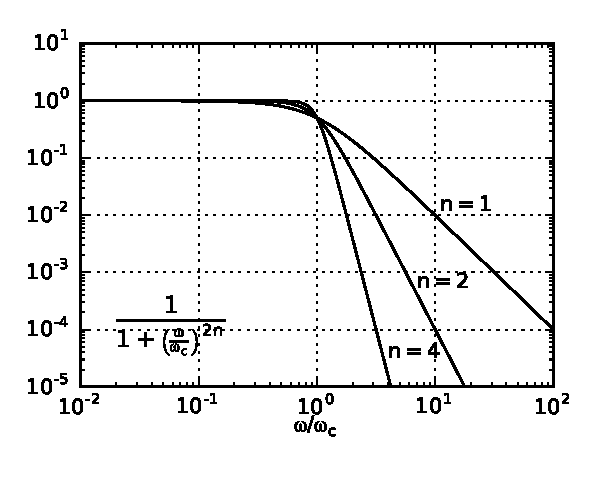
\includegraphics[scale=1.0]{figures/figure1}
\caption{Frequency response of the RBF-FD filter from eq. (\ref{eq:1DFourierSoln2}) for different values of $n$.}   
\label{fig:FrequencyResponse}
\end{figure}

The above Fourier analysis reveals how eq. (\ref{eq:1DSolution}) will behave under LTI assumptions.  For the GPS data considered in this paper, this assumption is not appropriate because neither the data uncertainties nor the sampling rates are constant. When the LTI conditions are not satisfied, it is no longer obvious how eq. (\ref{eq:1DSolution}) behaves or whether it can still be viewed as a low-pass filter with cutoff frequency $\omega_c$.  

We explore the behavior of eq. (\ref{eq:1DSolution}) under more general conditions. We continue to substitute $\lambda$ in eq. (\ref{eq:1DSolution}) with eq. (\ref{eq:VariableChange}), which changes our free parameter to $\omega_c$. Since we are no longer assuming a constant variance, we replace $\sigma^2$ in eq. (\ref{eq:VariableChange}) with a characteristic variance, $\bar{\sigma}^2$, which we define as
         
\begin{equation}
\frac{1}{\bar{\sigma^2}} = \frac{1}{N} \mathrm{tr}\left(\mathbf{C}_\mathrm{obs}^{-1}\right),
\end{equation}
where $N$ is the number of observations.  We now write our smoothed solution as

\begin{equation}\label{eq:1DSolution2}
\begin{split}
\mathbf{\bar{u}}_\mathrm{post} &= (\mathbf{C}_\mathrm{obs}^{-1} +   
                   \frac{1}{(2\pi\omega_c)^{2n}\bar{\sigma}^2}\mathbf{D}_n^T\mathbf{D}_n)^{-1}
                   \mathbf{C}_\mathrm{obs}^{-1}
                   \mathbf{u}_\mathrm{obs}
\\
\mathbf{C}_\mathrm{post} &= (\mathbf{C}_\mathrm{obs}^{-1} +   
                            \frac{1}{(2\pi\omega_c)^{2n}\bar{\sigma}^2}\mathbf{D}_n^T\mathbf{D}_n)^{-1}.
\end{split}
\end{equation}
The behavior of eq. (\ref{eq:1DSolution2}) can be revealed by analyzing the eigen decomposition of the matrix mapping $\mathbf{u}_\mathrm{obs}$ to $\mathbf{\bar{u}}_\mathrm{post}$,

\begin{equation}\label{eq:Kernel}
\mathbf{K} = (\mathbf{C}_\mathrm{obs}^{-1} + 
              \frac{1}{(2\pi\omega_c)^{2n}\bar{\sigma}^2}\mathbf{D}_n^T\mathbf{D}_n)^{-1}\mathbf{C}_\mathrm{obs}^{-1}.
\end{equation}
The eigenvalues of $\mathbf{K}$, $s_1, \dots, s_N$, are real and bounded between 0 and 1.  The eigenvectors, $\mathbf{v}_1, \dots,\mathbf{v}_N$, are real and, when $\mathbf{K}$ is symmetric (e.g. when $\mathbf{C}_\mathrm{obs} = \sigma^2 \mathbf{I}$), form an orthogonal basis set.  Each eigenvalue, $s_i$,  describes the amount that $\mathbf{v}_i$ will be shrunk under the mapping $\mathbf{K}$.  The eigenvectors associated with eigenvalues close to 1 can then be interpretted as components which are retained in $\mathbf{\bar{u}}_\mathrm{post}$. When the LTI conditions are satisfied, the above Fourier analysis reveals that $\mathbf{v}_1, \dots, \mathbf{v}_N$ are a set of orthogonal sinusoids and $s_1, \dots s_N$ are the coresponding frequency responses from eq. (\ref{eq:1DFourierSoln2}). In Figure \ref{fig:Demo1} and \ref{fig:Demo2} we show the eigen decomposition of $\mathbf{K}$ under four different conditions; 1) $\mathbf{K}$ is an LTI filter; 2) we do not assume the signal is periodic (i.e. $\mathbf{D}_n$ is not a periodic differentiation matrix); 3) The data uncertainty is not constant; 4) the data sampling rate is not constant. In all cases, the eigenvectors still resemble sinusoids and the eigenvalues still decay in a manner consistent with the frequency response function in eq. (\ref{eq:1DFourierSoln2}). Specifically, the eigenvectors associated with eigenvalues greater than or equal to 0.5 resemble sinusoids with frequencies less than or equal to $\omega_c$. The remaining eigenvectors resemble sinusoids with frequencies greater than $\omega_c$ and they have eigenvalues that are effectively 0.  We can conclude that eq. (\ref{eq:1DSolution2}) still effectively behaves as a low-pass filter with cutoff frequency $\omega_c$, even when the LTI conditions are not satisfied.  

We discuss additional features in the eigenvectors for $\mathbf{K}$ that further illuminate the behavior of eq. (\ref{eq:1DSolution2}).  When $\mathbf{D}_n$ is a periodic differentiation matrix (Figure \ref{fig:Demo1}A-C), $\mathbf{u}_\mathrm{post}$ is forced to be periodic.  If this assumption is not appropriate for the underlying signal then errors may be introduced at the domain edges (Figure \ref{fig:Demo1}A).  In figure \ref{fig:Demo1}D-F we show a smoothing demonstration and the eigen decomposition of $\mathbf{K}$ when we use a non-periodic differentiation matrix.  From Figure \ref{fig:Demo1}D, we can see that the smoothed solution is a much better prediction of the underlying signal at the edges.  When we drop the periodicity assumption, the smoothed solution tends to have its most extreme values at the edges.  This can be seen by inspecting the eigenvectors in Figure \ref{fig:Demo1}E, where the maximum or minimum values for each eigenvector tend to be at the edges of the domain.  In Figure \ref{fig:Demo2}A-C, we provide a demonstration where the data uncertainties are anomalously high from the time interval 0.2-0.5. Over this interval, the eigenvectors are elongated, which is desirable behavior because it means that $\mathbf{u}_\mathrm{post}$ will not contort to fit dubious data.  Altough not shown here, when the data uncertainty over the time interval 0.2 to 0.5 is increased to infinity, $\mathbf{u}_\mathrm{post}$ converges to a solution which is not significantly different from that shown in Figure \ref{fig:Demo1}.  One could then surmise that the RBF-FD filter can be used for extrapolation by treating the extrapolation points as data with infinite uncertainty.  In Figure \ref{fig:Demo2}D-C we provide a demonstration where the sampling rate decreases over time.  In this case, the eigenvectors resemble those in \ref{fig:Demo1}E, except that the amplitudes decrease where the data is more highly contentrated.  The lower amplitude in the eigenvectors reflects the fact that the solution is more tighly constrained.    

\begin{figure}
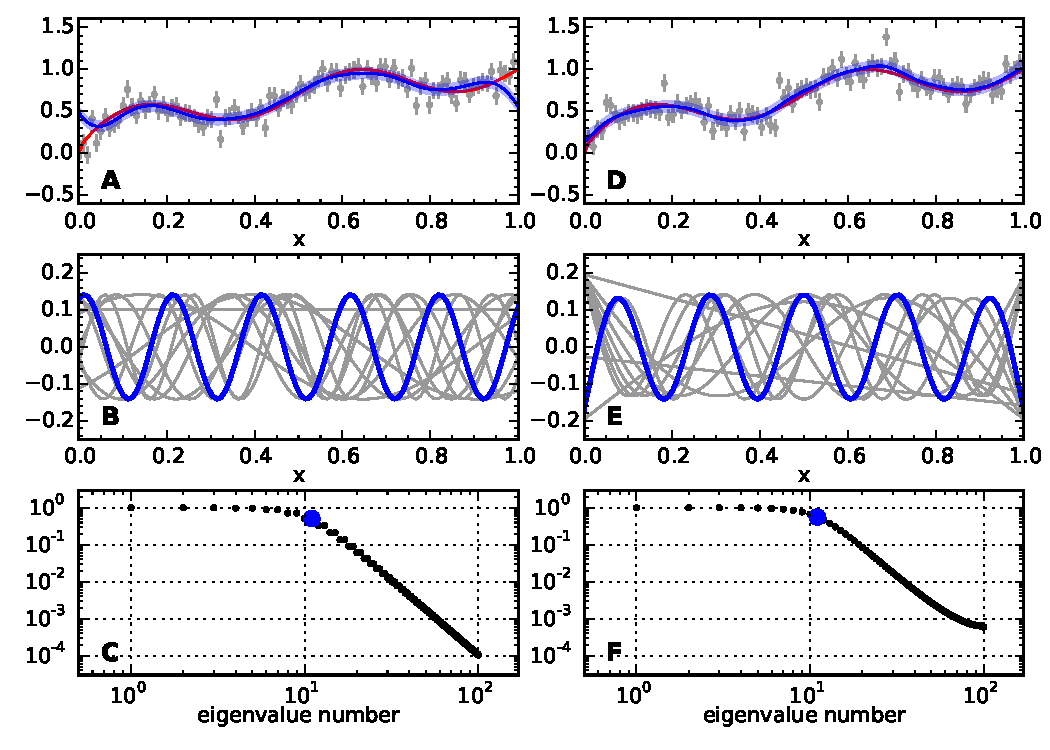
\includegraphics[scale=1.0]{figures/figure2}
\caption{eigenvectors and eigenvalues}   
\label{fig:Demo1}
\end{figure}

\begin{figure}
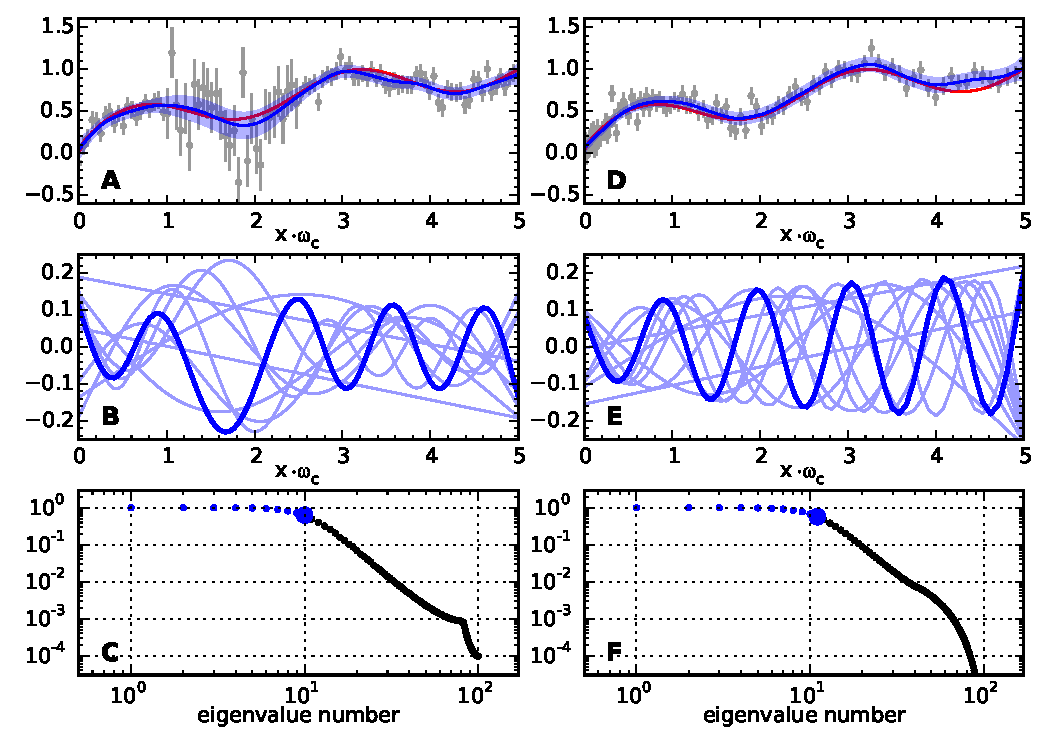
\includegraphics[scale=1.0]{figures/figure3}
\caption{eigenvectors and eigenvalues}   
\label{fig:Demo2}
\end{figure}

\subsubsection{Filtering in Higher Dimensions}\label{sec:SmoothingND} 
We expand our discussion to smoothing data which is observed in $d$-dimensional space.  The filtered solution is still given by eq. (\ref{eq:GeneralSolution}), and we consider the prior model

\begin{equation}
  \mathbf{L}_n \mathbf{u}_\mathrm{prior} = \mathbf{q}, \ \ \ \mathbf{q} \sim \mathcal{N}(0,\lambda^2)
\end{equation}  
where $\mathbf{L}_n$ is a differentiation matrix which approximates the operation 

\begin{equation}
  \sum_{i=1}^d\frac{\partial^n}{\partial x_i^n} 
\end{equation} 
and $n$ is an even integer. In general, we can construct $\mathbf{L}_n$ for arbitrarily spaced data with the strategy described in Section \ref{sec:Differentiating}. The corresponding prior covariance matrix is

\begin{equation}\label{eq:NDCovariance}
\mathbf{C}_\mathrm{prior} = \lambda^2\left(\mathbf{L}_n^T\mathbf{L}_n\right)^{-1}. 
\end{equation}           
Using the change of variables from eq. (\ref{eq:VariableChange2}), the solution in the time domain is

\begin{equation}\label{eq:NDSolution}
\begin{split}
\mathbf{\bar{u}}_\mathrm{post} &= (\mathbf{C}_\mathrm{obs}^{-1} +   
                   \frac{1}{(2\pi\omega_c)^{2n}\bar{\sigma}^2}\mathbf{L}_n^T\mathbf{L}_n)^{-1}\mathbf{C}_\mathrm{obs}^{-1}
                   \mathbf{u}_\mathrm{obs}
\\
\mathbf{C}_\mathrm{post} &= (\mathbf{C}_\mathrm{obs}^{-1} +   
                            \frac{1}{(2\pi\omega_c)^{2n}\bar{\sigma}^2}\mathbf{L}_n^T\mathbf{L}_n)^{-1}.
\end{split}
\end{equation}
If we again assume that the observation are regularly spaced, have constant variance, and $\mathbf{L}_n$ is the corresponding spectral differentiation matrix, then the $d$-dimensional discrete Fourier transform of $\mathbf{\bar{u}}_\mathrm{post}$ is 

\begin{equation}\label{eq:NDFourierSoln}
  \mathbf{\hat{u}}_\mathrm{post}(\omega_1, \dots, \omega_d) = 
  \frac{1}{1 + \left(\sum_{i=1}^d \left(\frac{\omega_i}{\omega_c}\right)^n\right)^2} \mathbf{\hat{u}}_\mathrm{obs}.
\end{equation}
The frequency response for eq. (\ref{eq:NDSolution}) can once again be recognized as a low-pass filter with cutoff frequency $\omega_c$.  In the limit as $n \to \infty$, the frequency response becomes a $d$-dimensional box which is zero for all the frequency tuples $(\omega_1,\dots,\omega_d)$ which have at least one component whos magnitude is greater than $\omega_c$.

\begin{figure}
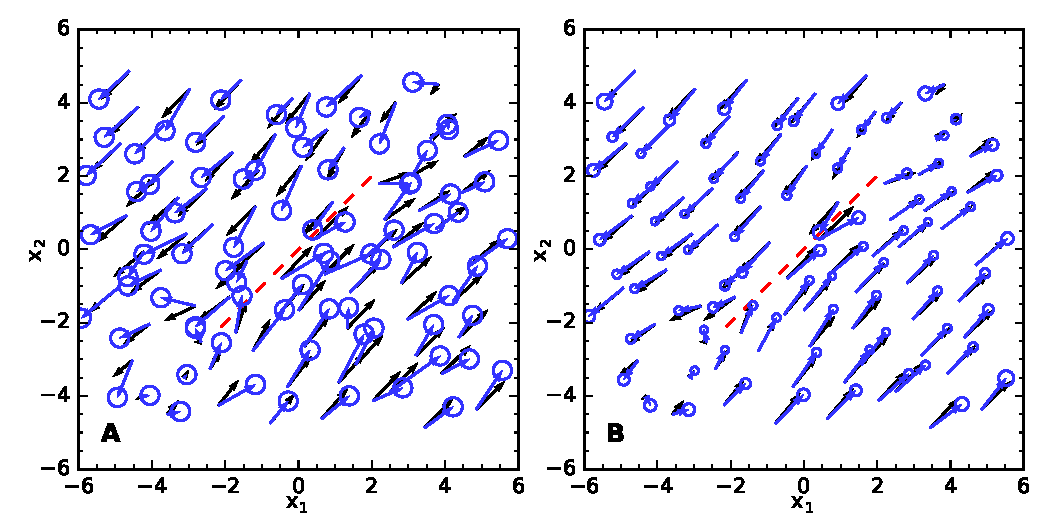
\includegraphics[scale=1.0]{figures/figure4}
\caption{eigenvectors and eigenvalues}   
\label{fig:Demo3}
\end{figure}

\section{Applications}\label{sec:Applications}

\subsection{Strain Rate in Southern California}\label{sec:ApplicationsSoCal}
give definition of strain
remark on how uncertainties are computed and also how they dont account for error in L

\subsection{Time Depenent Strain Rate in Cascadia}\label{sec:ApplicationsCascadia}

\section{Discussion and Conclusion}\label{sec:Discussion}
% discuss potential applications for slip models

% discuss how we remove errors like reference frame and seasonals

% discuss how this can be used for tikhonov regularization

\bibliographystyle{apalike}
\bibliography{mybib}  
 
\end{document}